% !TeX root = main.tex
% !TEX program = pdflatex

\chapter{Introducción}

\section{Contextualización del Cáncer}
\label{sec:context-cancer}

El cáncer\footnote{El cáncer es una de las principales causas de muerte a nivel mundial, afectando a millones de personas cada año. Según la Organización Mundial de la Salud (OMS), se estima que en 2020 hubo aproximadamente 19.3 millones de nuevos casos y 10 millones de muertes por cáncer en todo el mundo. La detección temprana y el tratamiento adecuado son cruciales para mejorar las tasas de supervivencia.} se ha convertido en uno de los mayores desafíos de la salud pública alrededor del mundo, esto es debido a su elevada incidencia y su mortalidad. Es una enfermedad que afecta a millones de personas cada año, y representa una de las principales causas de muertes en muchos países, independientemente del nivel de desarrollo de estos mismos. No solo tiene una repercusión sanitaria, el cáncer tiene muchas repercusiones tanto económicas como sociales, ya que impacta de forma directa en la calidad de vida de los pacientes. El tratamiento del cáncer requiere un enfoque que debe combinar la prevención, el diagnóstico precoz, un tratamiento eficaz y un seguimiento continuo, a lo largo de este proceso deben de estar implicados profesionales de distintas disciplinas dentro del propio sistema sanitario. 

\subsection{Definición General del Cáncer}
\label{sec:def-cancer}

Se podría definir el cáncer como un grupo extenso de enfermedades, que se distinguen por la proliferación descontrolada e irregular de células que tienen la habilidad de infiltrarse y destruir tejidos cercanos, o incluso de extenderse hacia otros órganos a través de procesos metastásicos\cite{WHO2025}. La base biológica de esta enfermedad se encuentra en cambios genéticos y epigenéticos, ya sean heredados u adquiridos, que alteran procesos del ciclo celular, como la apoptosis o la multiplicación celular. Estas alteraciones genéticas propician que las células desarrollen conductas invasivas y se propaguen sin restricciones, generando de esta manera tumores malignos en cualquier tejido u órgano. 

\subsection{Impacto Mundial del Cáncer: Epidemiología y Tendencias Globales}
\label{sec:impact-cancer}

\paragraph[short]{Estadísticas Mundiales de Incidencia y Prevalencia}
%\label{sec:global-statistics}

A nivel global, el cáncer es una de las enfermedades más frecuentes y una de las principales causas de mortalidad. Según datos proporcionados por GLOBOCAN 2020\cite{globocan2020}, se estimó que en dicho año se produjeron aproximadamente 19,3 millones de nuevos casos de cáncer en el mundo. Los tipos de cáncer más diagnosticados a nivel global son el cáncer de mama, pulmón, colorrectal, próstata y gástrico. La incidencia global continúa aumentando, principalmente debido al envejecimiento poblacional y al incremento en la prevalencia de factores de riesgo asociados al estilo de vida.

\paragraph[short]{Tendencias en la Incidencia del Cáncer}
%\label{sec:global-trends}
Las tendencias en la incidencia del cáncer muestran un aumento constante en la mayoría de las regiones del mundo, especialmente en países en desarrollo. Este incremento se atribuye a varios factores, incluyendo el envejecimiento de la población, la urbanización y la adopción de estilos de vida poco saludables, como el tabaquismo, el sedentarismo y dietas poco saludables. Además, se ha observado un aumento en la detección temprana y el diagnóstico de cáncer, lo que también contribuye al aumento aparente de casos\cite{Zhou2024}.
\subsection{Supervivencia y Mortalidad por Cáncer}
\label{sec:survival-mortality}


\paragraph[short]{Supervivencia y mortalidad según el tipo de cáncer}
% \label{sec:survival-mortality} 

Las tasas de supervivencia en cáncer varían considerablemente según el tipo específico y el estadio en el que se realiza el diagnóstico. Por ejemplo, el cáncer de mama presenta tasas de supervivencia a 5 años superiores al 80\% en países desarrollados gracias a la detección precoz y mejores tratamientos disponibles. En cambio, el cáncer de pulmón muestra tasas de supervivencia significativamente menores, inferiores al 20\%, principalmente debido a su diagnóstico tardío y la agresividad propia del tumor\cite{allemani2018global}. Otros tipos de cáncer con peor pronóstico incluyen el cáncer de páncreas, con una supervivencia a cinco años que raramente supera el 10\%, dada la dificultad en su detección temprana. 

\paragraph[short]{Tasas globales de mortalidad por cáncer}
% \label{sec:global-mortality} 

A nivel mundial, el cáncer constituye la segunda causa de muerte más común después de las enfermedades cardiovasculares, siendo responsable de aproximadamente uno de cada seis fallecimientos anuales en el mundo. En 2020, aproximadamente 10 millones de personas fallecieron por causa directa del cáncer. El cáncer de pulmón es el más letal, seguido del cáncer colorrectal y hepático, siendo estos tres tipos responsables de casi la mitad del total de muertes relacionadas con el cáncer\cite{Sung2021}. 

\subsection{Estadísticas del Cáncer en España}
\label{sec:stats-cancer-spain}

\paragraph{Casos nuevos diagnosticados anualmente}

En España, el cáncer continúa siendo uno de los problemas de salud pública más importantes, registrándose cada año aproximadamente 280.100 nuevos casos según el informe de la Sociedad Española de Oncología Médica (SEOM)  \cite{SEOM2025}. Esta cifra se prevé que continúe aumentando en las próximas décadas debido al envejecimiento de la población española y el impacto acumulativo de factores ambientales y hábitos de vida. 

\paragraph{Tipos más frecuentes de cáncer en España} 

En la población española, se han detectado los siguientes cánceres como los más frecuentes: cáncer colorectal, cáncer de próstata, cáncer de pulmón, cáncer de mama y cáncer de vejiga urinaria. En el caso de los hombres, dominan los cánceres de próstata, pulmón y colon, mientras que, en el caso de las mujeres, el cáncer más frecuente es el cáncer de mama, seguido por el cáncer de colon y el cáncer de pulmón, estos datos están condicionados en parte por los hábitos de vida establecidos y por las características demográficas particulares del país como indica la Sociedad Española de Oncología Médica (SEOM). 

\subsection{Factores Influyentes en la Incidencia del Cáncer}
\label{sec:influencing-factors} 

El cáncer es una enfermedad multifactorial, influenciada por factores demográficos, genéticos y ambientales, siendo fundamental identificar estos factores para establecer estrategias preventivas eficaces. 

\paragraph{Factores demográficos} 

Entre los factores demográficos más relevantes está la edad, ya que la mayoría de los tipos de cáncer tienen una incidencia notablemente mayor en personas mayores de 60 años, debido a la acumulación de mutaciones genéticas a lo largo de la vida. Asimismo, el sexo condiciona considerablemente la incidencia de ciertos tipos específicos de cáncer, como el cáncer de próstata, que es exclusivamente masculino, o el cáncer de mama, que presenta una mayor incidencia en mujeres\cite{cancer_risk_factors}. Por último, la herencia genética también representa un factor importante para algunos tipos de cáncer, como ocurre con el cáncer de mama y ovario en pacientes con mutaciones en los genes BRCA1 y BRCA2. 

\paragraph{Factores de riesgo asociados al estilo de vida} 

Diversos estudios han demostrado que los factores asociados al estilo de vida juegan un papel decisivo en la incidencia de cáncer. El tabaquismo constituye el principal factor de riesgo evitable para numerosos tipos de cáncer, especialmente cáncer de pulmón, cabeza y cuello, y vías urinarias\cite{restrepo1988relacion}. Otros factores relacionados con hábitos de vida son el consumo excesivo de alcohol, una dieta rica en grasas saturadas y pobre en fibra, la obesidad, el sedentarismo y la exposición prolongada al sol sin protección, factores todos ellos que incrementan significativamente el riesgo de desarrollar diferentes tipos de cáncer\cite{PAPPS2024}. Por ello, la prevención primaria, mediante cambios en el estilo de vida, representa una estrategia clave en la reducción del riesgo global y en la disminución de la incidencia de cáncer.

\subsection{Importancia de la Detección Temprana y el Tratamiento}
\label{sec:importance-early-detection}
La detección temprana del cáncer es crucial para mejorar las tasas de supervivencia y la calidad de vida de los pacientes. La identificación precoz de la enfermedad permite iniciar tratamientos más efectivos y menos invasivos, lo que puede llevar a una mayor probabilidad de curación o control de la enfermedad. Las estrategias de detección temprana incluyen programas de cribado poblacional, como mamografías para el cáncer de mama, colonoscopias para el cáncer colorrectal y pruebas de Papanicolaou para el cáncer cervical. Estos programas han demostrado reducir la mortalidad por cáncer en poblaciones específicas al facilitar diagnósticos en etapas más tratables\cite{usptf2023cancer}.
\subsection{Avances en la Investigación y Tratamiento del Cáncer}
\label{sec:advances-cancer-research}          
La investigación en cáncer ha avanzado significativamente en las últimas décadas, lo que ha llevado al desarrollo de nuevas terapias y enfoques de tratamiento. Los avances en la biología molecular y la genética han permitido identificar biomarcadores específicos que pueden predecir la respuesta a ciertos tratamientos, lo que ha llevado a la personalización de la terapia oncológica\cite{Hanahan2022}. Además, el desarrollo de terapias dirigidas y la inmunoterapia han revolucionado el tratamiento del cáncer\cite{Schreiber2021}, ofreciendo nuevas esperanzas para pacientes con tumores previamente considerados incurables. Estos avances no solo mejoran las tasas de supervivencia, sino que también reducen los efectos secundarios asociados con tratamientos más agresivos\cite{Mukherjee2010}.

\section{La Planificación Quirúrgica en Oncología}
\label{sec:oncology-surgical-planning}

\subsection{Concepto General de la Planificación Quirúrgica}
\label{sec:general-concept-surgical-planning}
La planificación quirúrgica se refiere al conjunto de procesos y estrategias empleadas por los equipos de clínicos para diseñar, optimizar y anticipar los pasos necesarios para llevar a cabo una intervención quirúrgica. Este proceso incluye no solo la identificación precisa de la patología a tratar, sino también la determinación detallada de las estructuras anatómicas implicadas, la evaluación de posibles riesgos y complicaciones, y la selección del abordaje quirúrgico más adecuado según el contexto clínico específico de cada paciente\cite{Gillies2020}. 

El objetivo principal de la planificación quirúrgica es maximizar la eficacia y seguridad del procedimiento, buscando eliminar o controlar la patología tumoral con la menor afectación posible de estructuras vitales adyacentes, preservando así al máximo la función de los órgano y tejidos sanos. Esto se traduce directamente en una mejora de la calidad de vida del paciente tras la cirugía, reduciendo significativamente los riesgos postoperatorios, la duración del periodo de recuperación y mejorando las tasas globales de supervivencia\cite{Birkmeyer2012}. 

Una planificación quirúrgica precisa y rigurosa resulta particularmente importante en cirugía oncológica, donde la exactitud en la identificación y delimitación tumoral puede ser determinante para conseguir resecciones completas, con márgenes libres adecuados, reduciendo el riesgo de recurrencias o metástasis futura\cite{NCCN2023}.

\subsection{El Papel Crucial de la Imagen Médica en la Planificación Quirúrgica}
\label{sec:medical-image-surgical-planning}

 

\paragraph{Técnicas y modalidades principales en imagen médica} 

En el ámbito de la planificación quirúrgica oncológica, las técnicas de imagen médica desempeñan un papel crucial al proporcionar información anatómica y funcional que permite evaluar la extensión tumoral, detectar lesiones secundarias y definir claramente los márgenes quirúrgicos. Actualmente, las modalidades de imagen más utilizadas son la tomografía computarizada (TC), la resonancia magnética (RM), la ecografía (US), la tomografía por emisión de positrones (PET) y la radiografía convencional (rayos X), cada una de ellas con características propias, ventajas y limitaciones según el tipo de cáncer, la localización anatómica y el objetivo clínico concreto. 

La tomografía computarizada (TC) es una técnica de imagen que emplea radiación de tipo ionizante (rayos X) para generar imágenes tridimensionales con una alta resolución anatómica. La TC permite identificar con precisión la localización, tamaño y características morfológicas de tumores sólidos, siendo especialmente útil en tumores pulmonares, óseos, cerebrales y hepáticos. Además, presenta las siguientes ventajas:  rapidez en adquisición y alta precisión en la detección de calcificaciones y lesiones óseas, aunque presenta una limitación a considerar al utilizar radiación ionizante, la cual es dañina para la salud\cite{image_guided_cancer_surgery}. 

La resonancia magnética (RM) produce imágenes complejas y muy detalladas mediante la interacción entre campos magnéticos intensos y ondas de radiofrecuencia, y muestra un buen contraste entre los tejidos blandos sin usar radiación ionizante. La RM resulta muy útil en la caracterización de los tumores, la valoración de la invasión local de los tumores, o la determinación de su extensión a partir de las diferentes secuencias de imagen (T1, T2 y difusión)\cite[-1.5cm]{Bortot2023}. A pesar de estas ventajas, posee unos tiempos de adquisición más largos que otras modalidades, presenta contraindicaciones en zonas donde la paciente lleve implantes metálicos o dispositivos médicos. 

La ecografía (ultrasonidos, US) es una prueba que se basa en la utilización de ondas acústicas de alta frecuencia para proporcionar imágenes en tiempo real del interior del cuerpo humano. Lo que la hace destacar es su utilización de imágenes en tiempo real, su carácter dinámico, su portabilidad y la ausencia de radiación. Se utiliza con frecuencia en el análisis de biopsias guiadas, el diagnóstico diferencial de lesiones superficiales (mama, tiroides), así como para la evaluación de lesiones hepáticas superficiales\cite[-2.2cm]{ESOBI2019}\cite{Hung2021}. La principal limitación de la ecografía es que depende del operador e incluye dificultades para evaluar las lesiones profundas o en los pacientes obesos. 

La tomografía por emisión de positrones (PET) es una modalidad de imagen nuclear que permite la evaluación funcional y metabólica mediante la administración de radiotrazadores. Habitualmente se combina con TC (PET/TC), integrando la información anatómica y funcional para mejorar el diagnóstico de metástasis, monitorización terapéutica y detección temprana de recidivas tumorales. Su principal limitación es la baja resolución anatómica y la exposición a radiación\cite{PETCTOncology2014}. 

La radiografía convencional (rayos X) utiliza radiación ionizante para obtener imágenes bidimensionales, siendo especialmente útil en la identificación rápida y económica de lesiones óseas, patologías pulmonares o metástasis óseas. Aunque su resolución espacial es menor en comparación con TC o RM, ofrece una rápida evaluación preliminar en múltiples escenarios clínicos. Sin embargo, debido a su naturaleza bidimensional, no proporciona información suficiente para una planificación quirúrgica precisa en casos complejos\cite{imagenologia_cancer}. 

Además de estas técnicas convencionales, otras modalidades relevantes en oncología incluyen la mamografía (modalidad especializada de rayos X para cáncer de mama), la endoscopia (para lesiones en tracto digestivo) y la tomografía computarizada por emisión de fotón único (SPECT), una técnica de medicina nuclear que aporta información funcional adicional. 

En resumen, cada técnica presenta ventajas e inconvenientes específicos, y la elección de una u otra dependerá del tipo de cáncer, la región anatómica, el objetivo diagnóstico y la información clínica requerida. La combinación y comparación de estas técnicas permite optimizar el diagnóstico y planificación terapéutica, siendo habitual en la práctica clínica utilizar varias modalidades de imagen complementarias para obtener información anatómica, funcional y metabólica integrada, mejorando así la precisión y seguridad en la planificación quirúrgica oncológica\cite{Fang2022}. 

\paragraph{Criterios de selección de modalidad según tipo de cáncer y localización}

La elección adecuada de la técnica o modalidad de imagen médica en oncología es crucial para obtener información clínica precisa que permita definir claramente la estrategia quirúrgica a seguir. Dicha elección depende de diversos factores clínicos, entre los que destacan el tipo de tumor, su localización anatómica, el objetivo diagnóstico, y las características particulares de cada paciente. Por ello, la selección de la técnica más apropiada requiere de un conocimiento profundo de las ventajas, limitaciones y especificidades diagnósticas de cada modalidad disponible. 

En tumores localizados en tejidos blandos y estructuras anatómicas complejas, como los tumores cerebrales, pélvicos, hepáticos o pancreáticos, la resonancia magnética (RM) suele ser la modalidad preferida debido a su excelente resolución de contraste y capacidad para diferenciar con precisión tejidos adyacentes. Además, la RM permite identificar con detalle las relaciones anatómicas del tumor con estructuras críticas, lo cual es esencial para minimizar riesgos durante la cirugía. También resulta especialmente útil en la evaluación de tumores en regiones donde la diferenciación precisa del margen tumoral condiciona significativamente el pronóstico del paciente, como en cáncer de próstata, tumores ginecológicos o cáncer hepático primario [14]. 

Por otro lado, la tomografía computarizada (TC) es frecuentemente la técnica de elección para tumores óseos, pulmonares, y en aquellos casos donde la rapidez diagnóstica y la alta resolución espacial sean prioritarias. Por ejemplo, la TC constituye la modalidad principal para la evaluación del cáncer de pulmón, facilitando la evaluación de lesiones pulmonares, adenopatías mediastínicas, e invasión ósea o pleural. También se utiliza rutinariamente en tumores óseos primarios o secundarios (metástasis óseas), dado que permite valorar con precisión la extensión local, destrucción ósea y afectación de estructuras adyacentes [19]. 

La ecografía (US) tiene su principal aplicación en lesiones superficiales o fácilmente accesibles mediante abordajes percutáneos, como cáncer de mama, tiroides, tumores hepáticos superficiales y ciertos tumores renales. Se utiliza comúnmente para procedimientos intervencionistas guiados por imagen, tales como biopsias o marcajes preoperatorios, gracias a su capacidad para visualizar estructuras en tiempo real sin exponer al paciente a radiación. Sin embargo, su uso está limitado en lesiones profundas o de difícil visualización por presencia de aire o estructuras óseas [15]. En cuanto a la tomografía por emisión de positrones (PET), habitualmente combinada con TC (PET/TC), su principal criterio de selección radica en la necesidad de información metabólica y funcional para evaluar la extensión tumoral sistémica y la actividad metabólica de la enfermedad. Su uso es especialmente relevante en linfomas, cáncer de pulmón, tumores gastrointestinales y melanoma, donde detectar precozmente metástasis o evaluar respuesta al tratamiento resulta esencial para una correcta planificación terapéutica. Por su capacidad para identificar focos de actividad tumoral a distancia, la PET/TC desempeña un papel crucial en el manejo del cáncer avanzado y en la planificación de abordajes quirúrgicos radicales o paliativos [16]. 

Finalmente, la radiografía convencional (rayos X), aunque limitada en términos de resolución espacial y anatómica en comparación con técnicas más avanzadas, continúa siendo una herramienta inicial útil para identificar lesiones óseas, especialmente en la detección rápida y económica de metástasis óseas y patologías pulmonares que requieran una valoración urgente inicial antes de recurrir a técnicas más específicas y precisas como TC o RM [17]. 

En definitiva, la elección de la modalidad de imagen más adecuada depende directamente de la patología concreta que se esté abordando, su localización anatómica, los objetivos clínicos específicos del estudio y las características del paciente. Habitualmente, la combinación de diferentes modalidades suele proporcionar información complementaria valiosa, mejorando significativamente la precisión diagnóstica y optimizando así la planificación quirúrgica en oncología [18]. 

Dada la relevancia y utilidad clínica de la resonancia magnética (RM) en la planificación quirúrgica oncológica, especialmente en la evaluación precisa de tejidos blandos, delimitación tumoral y valoración de estructuras anatómicas complejas, este trabajo se enfocará específicamente en el uso y optimización de esta modalidad de imagen. La selección de la RM responde a la necesidad de obtener imágenes con alto contraste anatómico, libres de radiación ionizante, lo que permite un análisis detallado del tumor y facilita una planificación quirúrgica más precisa, segura y personalizada para los pacientes. 

\subsection{Resonancia Magnética: Técnica de imagen fundamental en planificación quirúrgica}
\label{sec:challenges-surgical-planning}


\paragraph{Fundamentos técnicos de la RM} 

La resonancia magnética (RM) se basa en la propiedad física del spin nuclear, un fenómeno cuántico asociado a los protones de los átomos de hidrógeno. Al colocar un paciente dentro de un campo magnético estático (B0) generado por el equipo de RM, los protones de hidrógeno se alinean en paralelo o antiparalelo a dicho campo, creando una magnetización neta en la dirección del campo externo. Este fenómeno se representa en la Figura 1, donde se ilustra la orientación de los momentos magnéticos (protones) bajo la influencia de un campo magnético uniforme [20]. 

\begin{marginfigure}[-6cm]
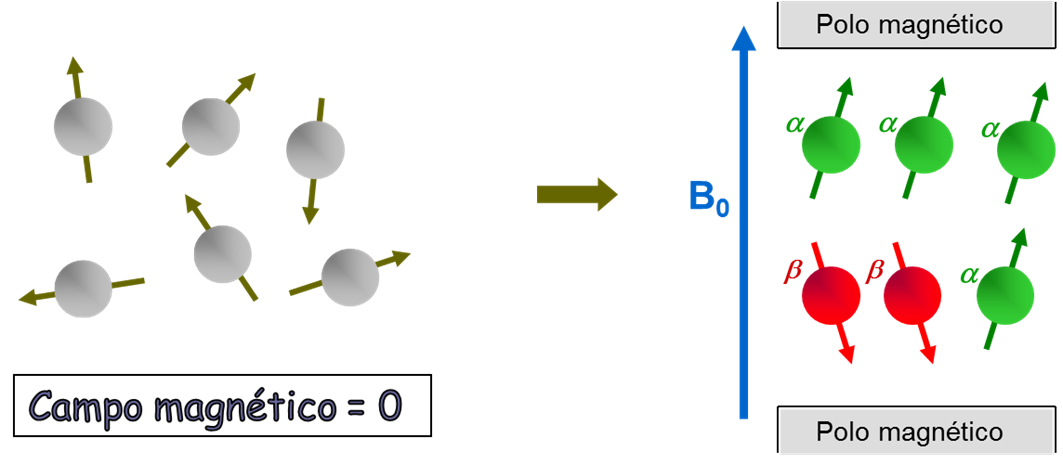
\includegraphics[width=\linewidth]{imagenes/campomagnetico.png}
% Imagen no encontrada. Actualiza la ruta o agrega el archivo correspondiente.
\caption{Representación esquemática de la orientación de los protones en presencia de un campo magnético estático.}
\label{fig:Esquema}
\end{marginfigure}

A continuación, se emite un pulso de radiofrecuencia (RF) con una frecuencia específica (frecuencia de Larmor), lo que provoca que los protones absorban energía y cambien su alineación. Cuando termina la excitación, los protones vuelven a su estado de equilibrio, emitiendo señales electromagnéticas que son captadas por las antenas del equipo de RM [21]. 

 

% 𝜔 = 𝛾 ∙ 𝐵0 

% donde: 

% 𝜔 es la frecuencia de Larmor (en Hz). 

% 𝛾 es la razón giromagnética del protón (𝛾 ≈ 42.58 MHz/T para el hidrógeno) 
% 𝐵0	es la intensidad del campo magnético (en Tesla) 

 

El retorno a la alineación original se describe mediante dos tiempos de relajación: 

Tiempo de Relajación Longitudinal (T1): Representa el tiempo que tardan los protones en recuperar su alineación con el campo magnético externo. 

Tiempo de Relajación Transversal (T2): Describe la pérdida de coherencia entre los protones debido a interacciones entre ellos. 

Estos parámetros determinan el contraste de la imagen y permiten la diferenciación entre distintos tipos de tejidos. 

\begin{figure}[hbtp]
  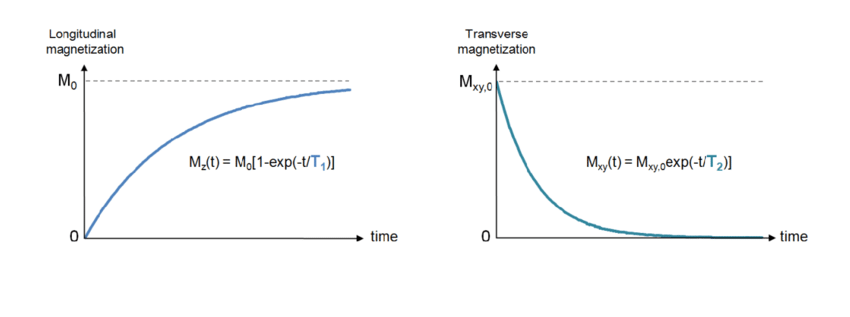
\includegraphics[width=\linewidth]{imagenes/Relaxation-rates-of-longitudinal-magnetization-1-T1-and-transverse-magnetization-1-T2.png}
  \caption{Recuperación de la magnetización longitudinal (T1) y el decaimiento de la magnetización transversal (T2).}
  %\setfloatalignment{t}% forces caption to be bottom-aligned
  \label{fig:T1yT2}
\end{figure}


